\documentclass[12pt,a4paper]{standalone}
\usepackage{tikz}
\usetikzlibrary{calc}
\usetikzlibrary{scopes}

\begin{document}
\def\camera#1#2{
\begin{scope}[shift={#1}, rotate=#2]
    \draw [fill=black](0,0) -- (2,2.5) -- (-2,2.5) -- cycle;
    \draw [fill=white,ultra thick](0,0) circle (1);
\end{scope}
}

% #1 shift #2 width #3 height #4 label critical point #5 label index #6 label extender #7 label length
\def\extender#1#2#3#4#5#6#7{
  
  \begin{scope}[shift={#1}]
    \def \markwidth {.2};
    \def \width {#2};
    \def \height {#3};
    % the indexratio is the ratio of the height of the index mark relative to the height of the extender
    \def \indexratio {.75};
    \coordinate (extender-crit) (0,0);
    \coordinate (extender-length) ($(extender-crit) + (0,\height)$);
    
    % mark for critical point
    \draw ($(extender-crit) - (\markwidth, 0)$) -- ($(extender-crit) + (\markwidth,0)$);
    
    % label critical point
    \draw ($(extender-crit) + (\markwidth,0)$) node[right]{#4};
    
    % mark for length
    \draw ($(extender-crit) + (- \markwidth, \height)$) -- ($(extender-crit) + (\markwidth,\height)$);
    
    % label length
    \draw ($(extender-crit) + (\markwidth, \height)$) node[right] {#7};

    % label extender
    \draw ($(extender-crit) + (2 * \markwidth,0.5 * \height)$) node[right] {#6};

    % draw index only if there is a nonempty label
    \def\temp{#5}\ifx\temp\empty
    
    \else
    % mark for index
    \draw ($(extender-crit) + (- \markwidth, \indexratio * \height)$) -- ($(extender-crit) + (\markwidth, \indexratio * \height)$);

    % label index
    \draw ($(extender-crit) + (2 * \markwidth, \indexratio * \height)$) node {#5};
    \fi
   
    
    % extender from critical point to length
    \draw (extender-crit) -- ($(extender-crit) + (\width,0)$)
                          -- ($(extender-crit) + (\width, \height)$)
                          -- ($(extender-crit) + (0, \height)$);

                      
  \end{scope}
}

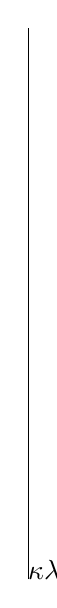
\begin{tikzpicture}
  \draw (0,0) -- (0,7);
  \extender{(0,3)}{-0.5}{3}{$\kappa$}{$\lambda$}{$F$}{$\gamma$};
  \extender{(0,2)}{-1}{5}{}{}{}{};

\end{tikzpicture}
\end{document}
